\documentclass{article}
\usepackage[utf8]{inputenc}
\usepackage{titling}
\usepackage{graphicx}
\usepackage{xcolor}
\usepackage[colorlinks=true,linkcolor=darkgray]{hyperref}
\usepackage[spanish]{babel}


\title{Práctica 5: PGP y Protocolos}
\author{Cristina Díaz García}
\date{Enero 2019}

\renewcommand\maketitlehooka{\null\mbox{}\vfill}
\renewcommand\maketitlehookd{\vfill\null}


\begin{document}

\addcontentsline{toc}{section}{Índice general}

\begin{titlingpage}
\maketitle
\end{titlingpage}

\newpage

\tableofcontents

\newpage

\section{Análisis del protocolo TELNET}

\begin{center}
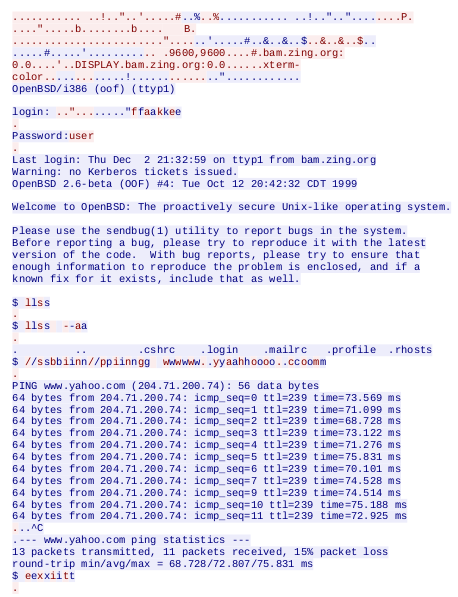
\includegraphics[scale=0.5]{images/telnet.png}
\end{center}

\begin{enumerate}
\item ¿Qué usuario y contraseña se ha aplicado para acceder al servidor de Telnet
192.168.0.1?

\textbf{usuario:} fake\\
\textbf{contraseña:} user

\begin{center}
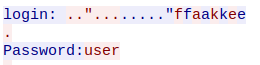
\includegraphics[scale=0.5]{images/login.png}
\end{center}
\item ¿Qué sistema operativo se está aplicando en el servidor?

Linux.

\begin{center}
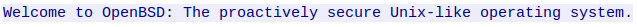
\includegraphics[scale=0.5]{images/linux.png}
\end{center}
\item ¿Qué comandos ha ejecutado el cliente en el servidor telnet?

ls\\
ls -a\\
/sbin/ping www.yahoo.com\\
Ctrl+C\\
exit\\

\begin{center}
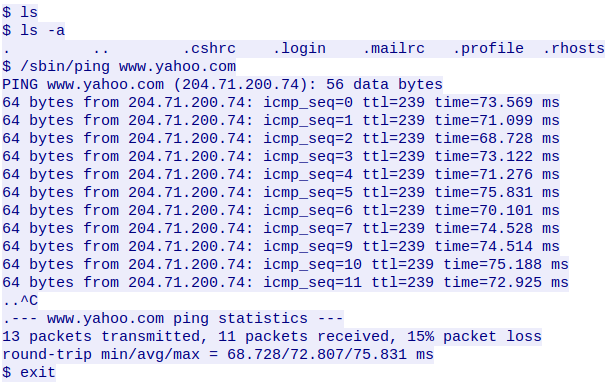
\includegraphics[scale=0.5]{images/command.png}
\end{center}
\end{enumerate}


\newpage

\section{Análisis del protocolo SSH}

\begin{enumerate}
\item ¿A partir de qué paquete comienza a cifrarse el tráfico de red?

A partir del 13º paquete.

\begin{center}
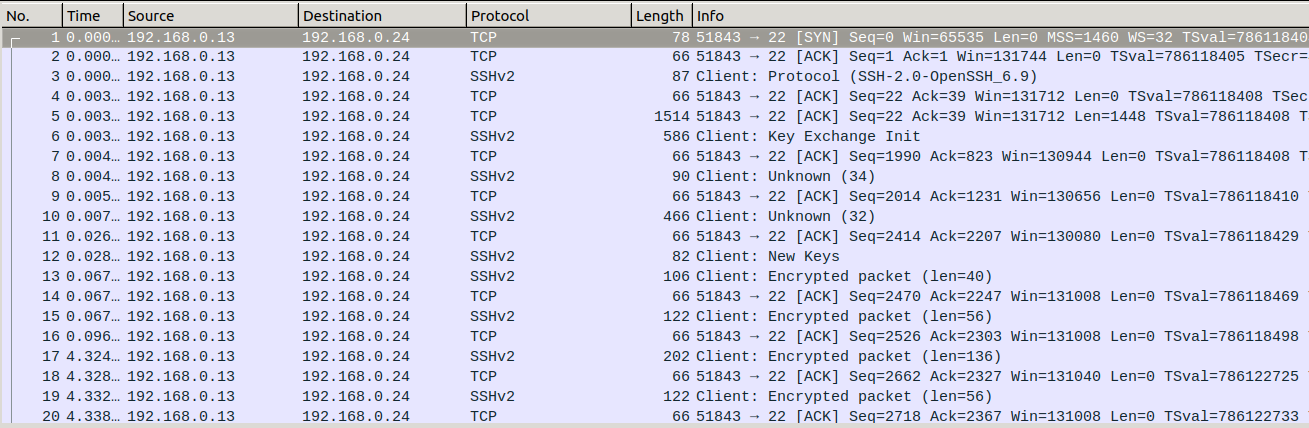
\includegraphics[scale=0.3]{images/ssh.png}
\end{center}
\item ¿A qué nivel se aplica el cifrado del protocolo SSH? Es decir, ¿se aplica el
cifrado a los protocolos de red (IP, TCP, etc.), a las capas superiores, o a
ambos?

A la capa de aplicación.

\begin{center}
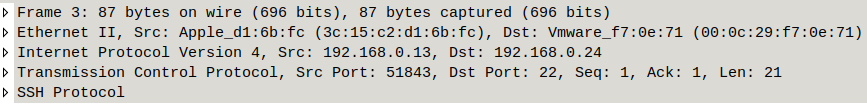
\includegraphics[scale=0.3]{images/capas.png}
\end{center}
\item ¿Es posible ver alguna información sobre credenciales de seguridad como
puede ser el usuario y la contraseña?

No, ya que está cifrado.
\end{enumerate}

\end{document}